\documentclass[a4paper]{article}
\usepackage[utf8]{inputenc}
\usepackage[UKenglish]{isodate}
\usepackage{parskip}

\usepackage{tikz}
\usepackage{minted}
\usetikzlibrary{positioning, fit, calc, arrows, shapes, arrows.meta}

\author{
Andreas Abild Mortensen \\
\texttt{anmor16@student.sdu.dk}
\and
Samuel Valdemar Grange \\
\texttt{sagra16@student.sdu.dk}
\and
Mads Grau Kristensen \\ 
\texttt{mkris16@student.sdu.dk} \\
\rule{5.5cm}{0.3mm}
}

\def§#1§{\texttt{#1}}

\usepackage{array}
\usepackage{listings}

\let\tt\texttt

\title{Bachelor Assignment 1}

\date{February 2019}


\definecolor{dkgreen}{rgb}{0,0.45,0}
\definecolor{gray}{rgb}{0.5,0.5,0.5}
\definecolor{mauve}{rgb}{0.30,0,0.30}

% Default settings for code listings
% Default settings for code listings
\lstset{frame=tb,
  language=Java,
  aboveskip=3mm,
  belowskip=3mm,
  showstringspaces=false,
  columns=flexible,
  basicstyle={\small\ttfamily},
  numbers=left,
  numberstyle=\footnotesize,
  keywordstyle=\color{dkgreen}\bfseries,
  commentstyle=\color{dkgreen},
  stringstyle=\color{mauve},
  frame=single,
  breaklines=true,
  breakatwhitespace=false
  tabsize=1
}

\begin{document}

\maketitle

\section{Introduction}
In this project we implemented a symbol table based on specifications from the project description. This symbol table will later be used as part of the front-end for our compiler.

\section{Problem}
In this assignment we are to implement one of the modules for the frontend of our compiler. The module we have implemented is a symbol table tree (lets call this \textbf{STT}).
The \textbf{STT} is a variable child tree, where each node contains a hash table, wherein every bucket of the hash tables contains a linked list of $(name, value)$ pairs.
The relationship is that every child can see the parent, but the parent cannot see the child; A one-way relationship.\\
We will be able to use the table to check for same-scope collisions and to look-up the "nearest" variable, in respect to the scope.

\section{Implementation}
We make use of recursion for parent table name look up, which we find more elegant than an iterative approach.
Moreover the code is well commented, so the code-inspector should have an easy time following the behaviour.
We use NULL extensively, to either indicate failure or to perform an "Item has not been allocated" check.
Finally we do account for potential stack allocated strings as input to the \textit{putSymbol} function (they may change later, but the address will remain the same), by internally allocating memory for the new string in the function itself (this may be subject to change in future assignments, but now the feature is there if we ever need to put a symbol from the stack).
Finally we naively return NULL's on errors, this may also be subject for change in future assignments since the symbol table code may be altered.

\begin{figure}
    \centering
    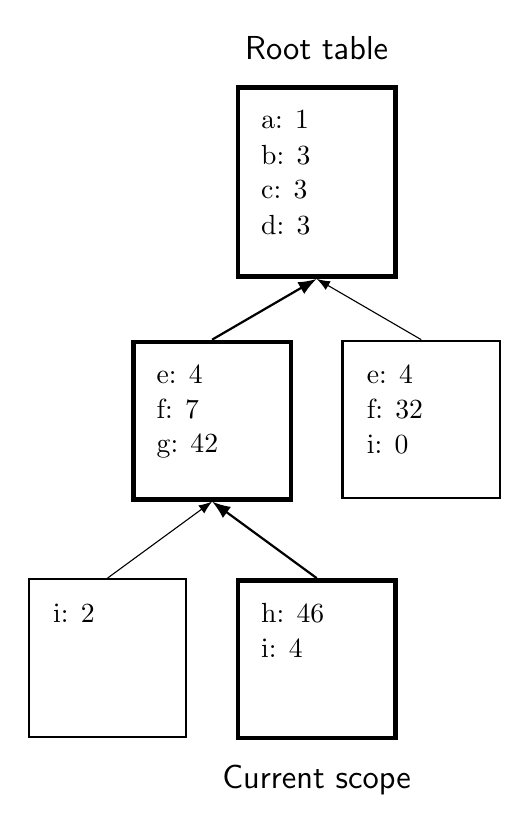
\begin{tikzpicture}[]
    \node (root table) at (0,0) [draw,ultra thick,minimum width=2cm,minimum height=2.4cm] {};
    
    \node[below=2cm of root table.west, xshift=-0.3cm] (1 table) [draw,ultra thick,minimum width=2cm,minimum height=2cm] {};
    
    \node[below=2cm of root table.east, xshift=0.3cm] (2 table) [draw,thick,minimum width=2cm,minimum height=2cm] {};
    
    \draw[-Latex, thick] (1 table.north) -- (root table.south) {};
    \draw[-Latex] (2 table.north) --  (root table.south) {};
    
    \node[below=2cm of 1 table.west, xshift=-0.3cm] (1-1 table) [draw,thick,minimum width=2cm,minimum height=2cm] {};
    \node[below=2cm of 1 table.east, xshift=0.3cm] (1-2 table) [draw,ultra thick,minimum width=2cm,minimum height=2cm] {};
    
    \draw[-Latex] (1-1 table.north) -- (1 table.south) {};
    \draw[-Latex, thick] (1-2 table.north) -- (1 table.south) {};
    
    \node[below=.2cm of 1-2 table] {\large \sffamily Current scope};
    \node[above=.2cm of root table] {\large \sffamily Root table};
    
    \node[xshift=.2cm, below=.2cm of root table.north west, anchor=north west] (a) {a: 1};
    \node[below=.2cm of a.west, anchor=north west] (b) {b: 3};
    \node[below=.2cm of b.west, anchor=north west] (c) {c: 3};
    \node[below=.2cm of c.west, anchor=north west] (d) {d: 3};
    
    \node[xshift=.2cm, below=.2cm of 1 table.north west, anchor=north west] (e1) {e: 4};
    \node[below=.2cm of e1.west, anchor=north west] (f1) {f: 7};
    \node[below=.2cm of f1.west, anchor=north west] (g1) {g: 42};
    
    \node[xshift=.2cm, below=.2cm of 2 table.north west, anchor=north west] (e1) {e: 4};
    \node[below=.2cm of e1.west, anchor=north west] (f1) {f: 32};
    \node[below=.2cm of f1.west, anchor=north west] {i: 0};
    
    \node[xshift=.2cm, below=.2cm of 1-2 table.north west, anchor=north west] (h1-2) {h: 46};
    \node[below=.2cm of h1-2.west, anchor=north west] {i: 4};
    
    \node[xshift=.2cm, below=.2cm of 1-1 table.north west, anchor=north west] (h1-1) {i: 2};
\end{tikzpicture}
    \caption{Illustration of how our tables are set up. The table with thick borders are the tables in which we would search for symbols, if our scope is as shown.}
    \label{fig:symboltable}
\end{figure}

\section{Testing Framework}
In this section we will be introducing our testing framework for this assignment and future ones.
We will only be elaborating on this framework in the first assignment, since future ones will be
 (almost) identical.\\
Our testing framework operates in a simple way. We will show how it works using a step-by-step algorithm and a visual representation.\\
\begin{enumerate}
    \item Initialize a FIFO queue
    \item For each test to be performed:
    \begin{enumerate}
        \item Add the 2-tuple of the test function and the test function's input to the queue
        \item Increment the queue item count by one
    \end{enumerate}
    \item For item in the queue:
    \begin{enumerate}
        \item Dequeue an element
        \item Call the function (the first element of the 2-tuple) with the argument (the second element of the 2-tuple)
        \item Print the result of the test function
    \end{enumerate}
\end{enumerate}
The idea behind testing with a framework (queue) is that it is much cleaner and easier to work with (from the developers perspective),
and much easier to read and understand. The code to add a test looks like the following (omitting the specific function and argument):
\begin{minted}{c}
appendTask(queue, testFunction, "Test message", (void*)testArgument);
\end{minted}
It should be noted that since C does not support any modern practices (curried functions in particular), we resort to having the argument stored with the function itself. The void pointer argument allows us to handle \textbf{Any} imaginable input (a list of structs allows complex inputs), and then cast them in the function body.

\begin{figure}
    \centering
    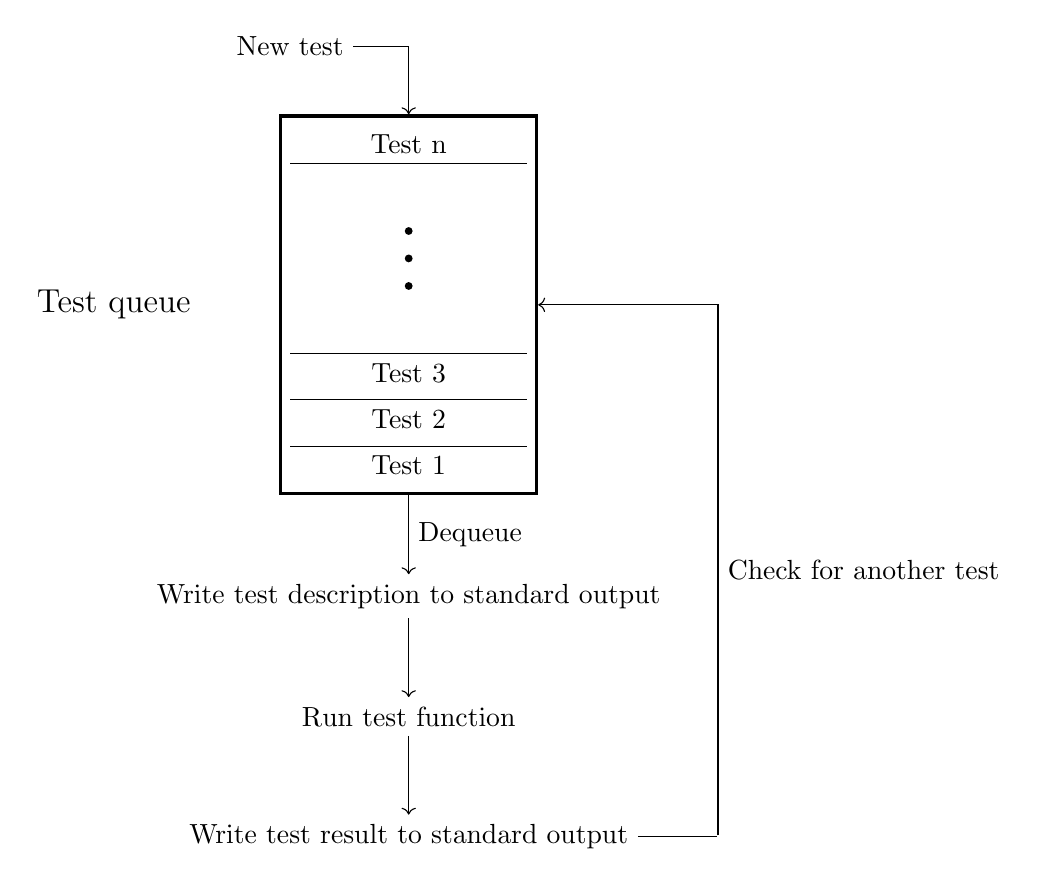
\begin{tikzpicture}[]
  \node[minimum width=3cm] (test 1) {Test 1};
  \node[above=.1cm of test 1, minimum width=3cm] (test 2) {Test 2};
  \node[above=.1cm of test 2, minimum width=3cm] (test 3) {Test 3};
  \node[above=3cm of test 2, minimum width=3cm] (test n) {Test n};
  
  \node [draw=black, very thick, fit=(test 1) (test n)] (stack) {};
  
  \draw(test 1.north west)--(test 1.north east);
  \draw(test 2.north west)--(test 2.north east);
  \draw(test 3.north west)--(test 3.north east);
  \draw(test n.south west)--(test n.south east);
  
  \node[above=.8cm of test 3] [circle,fill,inner sep=1pt]{}; 
  \node[above=1.15cm of test 3] [circle,fill,inner sep=1pt]{}; 
  \node[below=.8cm of test n] [circle,fill,inner sep=1pt]{};
  
  \node[above=1cm of test n.west] (new test) {New test};
  
  \draw[->, to path={-| (\tikztotarget)}]
    (new test) edge (stack.north);
    
  \node [left=of stack] {\large Test queue};
  
  \node[below=of stack] (test description) {Write test description to standard output};
  \node[below=of test description] (test run) {Run test function};
  \node[below=of test run] (test result) {Write test result to standard output};
  
  \draw[->] (stack.south) -- (test description) node[midway, anchor=west] {Dequeue};
  \draw[->] (test description.south) -- (test run);
  \draw[->] (test run.south) -- (test result);
  
  \node[right=of test result.east, inner sep=0, outer sep=0] (help) {};
  
  \draw[->] (test result.east) -- (help) |- (stack.east) node[pos=0.25, anchor=west] {Check for another test};
\end{tikzpicture}
    \caption{Illustration of the testing framework. Tests are put in a queue. Each test are dequeued and run in the order they were put in the queue}
    \label{fig:my_label}
\end{figure}

\section{Testing}
\begin{table}[H]
    \centering
    \newcolumntype{L}[1]{>{\raggedright\let\newline\\\arraybackslash\hspace{0pt}}m{#1}}
    \newcolumntype{C}[1]{>{\centering\let\newline\\\arraybackslash\hspace{0pt}}m{#1}}
    \begin{tabular}{|C{3cm}|L{3cm}|L{3cm}|C{1.5cm}|}
        \hline
        Test Name & Test Performed & Motivation for test & Passed / Failed \\
        \hline
        addItemsTest & Adds 50 items to a table. & We need to make sure that we can properly insert items into the symbol table. This test only checks that we do not encounter errors when inserting.  & Passed\\
        \hline
        getSymTest & Tests that the items inserted by \tt{addItemsTest} have been inserted correctly. & This test checks that the values from the previous test have been inserted correctly by trying to get one of the inserted items. & Passed\\
        \hline
        putRootTest & Adds an item to the root node in the Symbol table tree. & Not as much of a test but more of a preamble for the next text. & Passed\\
        \hline
        getRootFromChildTest & Tests that items in the root table can be found from child nodes. & We want to check if we can find items from parent tables by calling \tt{getSymbol()} on a child node, expecting the algorithm to traverse the tree until a match is found. & Passed\\
        \hline
        dumpTest & Runs \tt{dumpSymbolTable()} on a small tree of 2 nodes. The user must manually confirm that the information printed by the functions is correct. & We do this to check whether the table looks correct or not. Additionally it may segfault, meaning we may not be able to access all elements or something was not set to NULL. & Passed\\
        \hline
        putCollision & Runs \tt{putCollision()}; inserting two duplicate named items into the root node & We do this to check for collisions, we should return an error on collision. & Passed\\
        \hline
    \end{tabular}
\end{table}
If any tests fail, we expect either the wrong result which results in a failure message or a segfault. In any case, the probability of a successful implementation is increased by running the tests.

\section{How to run}
Since our compiler is not ready to compile anything yet, we exclusively run the tests.
The tests are compiled with the module they should test (hence they don't invoke any separately compiled binary for the symbol module).
We run our tests using CMake (running the CMakeFiles).\\
The tests for this project can be built following the instructions:
\begin{enumerate}
    \item Go to the tests folder.
    \item Run the shell script \textit{build.sh} (./build.sh)
    \item Run the tests (./tests)
\end{enumerate}
If preferred a pre-made Makefile can be found and used in the folder /tests/symbol/Makefile. It can be used by invoking it with \textbf{make all} and then run by executing \textbf{./tests}.


\newpage
\section{Source Code}
\subsection{Compiler files}
\subsubsection{symbol.h}
\begin{minted}{c}
#define HashSize 317

#include <stdio.h>
#include <string.h>
#include <stdlib.h>
#include <malloc.h>

#include "memory.h"

/* SYMBOL will be extended later.
   Function calls will take more parameters later.
*/

typedef struct SYMBOL {
  char *name;
  int value;
  struct SYMBOL *next;
} SYMBOL;

typedef struct SymbolTable {
    SYMBOL *table[HashSize];
    struct SymbolTable *next;
} SymbolTable;

int Hash(char *str);

SymbolTable *initSymbolTable();

SymbolTable *scopeSymbolTable(SymbolTable *t);

SYMBOL *putSymbol(SymbolTable *t, char *name, int value);

SYMBOL *getSymbol(SymbolTable *t, char *name);

void dumpSymbolTable(SymbolTable *t);
\end{minted}

\subsubsection{symbol.c}
\begin{minted}{c}
//
// Created by valde on 2/1/19.
//

#include "symbol.h"

int Hash(char *str){
    //If garbage is given
    if (str == NULL) {
        return -1;
    }

    size_t len = strlen(str);

    //If no chars, no need to run though
    if (len == 0) {
        return -1;
    }

    int sum = (int)str[0];

    //Start at 1, we initial the sum for first character above
    for (int i = 1; i < len; i++) {
        //Shift
        sum = sum << 1;
        //Add to sum
        sum = sum + (int)str[i];
    }

    return sum % HashSize;
}

SymbolTable *initSymbolTable() {
    //Create the initial table
    SymbolTable *table = NEW(SymbolTable);

    //Set next to null
    table->next = NULL;

    //Set all entries to NULL
    for (int i = 0; i < HashSize; i++) {
        (table->table)[i] = NULL;
    }

    return table;
}

SymbolTable *scopeSymbolTable(SymbolTable *t) {
    //Error handling
    if (t == NULL) {
        return NULL;
    }

    //New table and put old table in new tables next
    SymbolTable* htable = initSymbolTable();
    htable->next = t;
    return htable;
}

SYMBOL *putSymbol(SymbolTable *t, char *name, int value) {
    //Error stuff
    if (t == NULL || name == NULL) {
        return NULL;
    }

    //First we find the hash position
    int pos = Hash(name);

    //Then we find table root node of our desired item hash
    SYMBOL* current_node = t->table[pos];
    SYMBOL* parent_node = NULL;

    //Traverse until we find empty next
    while (current_node != NULL) {
        //Abort if we encounter a duplicate
        if (strcmp(name, current_node->name) == 0) {
            fprintf(stderr, "\nVariable declared in same scope %s same scope\n", name);
            fflush(stderr);
            return NULL;
        }
        
        parent_node = current_node;
        current_node = current_node->next;
    }

    //Node has been found, init it
    current_node = NEW(SYMBOL);
    current_node->next = NULL;

    //Allocate new space for the name (the given name is an R-value
    current_node->name = (char*)malloc(sizeof(char) * strlen(name));
    strcpy(current_node->name, name);

    current_node->value = value;
    
    //If parent node is not NULL we have to adjust the parent's next
    if (parent_node != NULL) {
        parent_node->next = current_node;
    } else {
        t->table[pos] = current_node;
    }

    //Node created and inited, we are done
    return current_node;
}

SYMBOL *getSymbol(SymbolTable *t, char *name) {
    //Error checking
    if (t == NULL || name == NULL) {
        return NULL;
    }

    //We hash name to find a matching bucket
    int bucketIndex = Hash(name);

    //Get the bucket
    SYMBOL *bucket = (t->table)[bucketIndex];

    //If bucket is NULL, we continue looking in next table
    if (bucket == NULL) {
        //We check if this is the root node, if yes we return NULL
        if (t->next == NULL) {
            return NULL;
        } else {
            //Recurse if we still have parents to look in
            return getSymbol(t->next, name);
        }
    }

    //We traverse the linked list for a match if a bucket is found
    while (strcmp(name, bucket->name) != 0) {
        //If the bucket is unallocated, we cannot find what we seek in this scope
        //Thus we must continue in the next scope
        if (bucket->next == NULL) {
            break;
        }

        //If there is not a match we continue looking in the linked list
        bucket = bucket->next;
    }

    //A bit of boilerplate, but if the name is not found in this scope, we look upwards again
    //We check if this is the root node, if yes we return NULL
    if (strcmp(name, bucket->name) == 0) {
        return bucket;
    } else if (t->next == NULL) {
        return NULL;
    } else {
        //Recurse if we still have parents to look in
        return getSymbol(t->next, name);
    }
}

void dumpSymbolTable(SymbolTable *t) {
    //Error check
    if (t == NULL) {
        return;
    }

    //We have our current node we are looking at
    SymbolTable *current_table = t;

    int tableNum = 0;
    //While the table we are looking at is allocated (aka it exists)
    while (current_table != NULL) {
        printf("We are looking at table %i:\n", tableNum);
        //We print our while whole table bucket wise
        for (int i = 0; i < HashSize; i++) {
            //This is the i'th symbol root node
            SYMBOL *current_symbol = (current_table->table)[i];

            if (current_symbol != NULL) {
                printf("At bucket %i we have the values:\n", i);
            }

            //We keep printing the contents of the linked list elements as long as they exist
            while (current_symbol != NULL) {
                //We print the contents of this node
                printf("name: %s, value: %i\n", current_symbol->name, current_symbol->value);

                //We prepare the next level
                current_symbol = current_symbol->next;
            }
        }

        //We proceed to the next table
        current_table = current_table->next;
        tableNum++;
    }
}
\end{minted}

\subsubsection{memory.h}
\begin{minted}{c}
void *Malloc(unsigned n);

#define NEW(type) (type *)Malloc(sizeof(type))
\end{minted}

\subsubsection{memory.c}
\begin{minted}{c}
#include <stdio.h>
#include <malloc.h>
#include <stdlib.h>

void *Malloc(unsigned n)
{
  void *p;
  if(!(p = malloc(n)))
  {
    fprintf(stderr,"Malloc(%d) failed.\n",n);
    fflush(stderr);
    abort();
  }
  return p;
}
\end{minted}

\subsection{Testing files}

\subsubsection{test.h}
\begin{minted}{c}
//
// Created by valde on 2/2/19.
//

#ifndef TESTS_TEST_H
#define TESTS_TEST_H

#include <stdio.h>
#include <malloc.h>
#include <string.h>

#include "queue.h"

typedef struct {
    char* taskName;
    int (*f)(void*);
    void *arg;
} Task;

void appendTask(Queue *q, int (*fnc)(void*), char *name, void *arg);
void runTaks(Queue *q);

#endif //TESTS_TEST_H
\end{minted}

\subsubsection{test.c}
\begin{minted}{c}
#include "test.h"


void evaluateTest(int result) {
    if (result == 0) {
        printf ("\033[31m FAILED \033[0m\n");
    } else if (result == 2) {
        printf ("\033[33m PENDING \033[0m\n");
    } else {
        printf ("\033[32m OK \033[0m\n");
    }
}

void appendTask(Queue *q, int (*fnc)(void*), char* name, void* arg) {
    Task *t = (Task*)malloc(sizeof(Task));

    t->f = fnc;
    t->taskName = (char*)malloc(sizeof(char) *strlen(name));
    strcpy(t->taskName, name);
    t->arg = arg;

    addElement(q, t);
}

void runTaks(Queue *q) {
    size_t max_size = q->remaining_elements;

    for (int i = 0; i < max_size; i++) {
        Task *t = (Task*)dequeue(q);

        printf("[%i/%i] %s -> ", max_size - q->remaining_elements, max_size, t->taskName);
        evaluateTest(2);
        fflush(stdout);

        int o = t->f(t->arg);

        printf("[%i/%i] %s -> ", max_size - q->remaining_elements, max_size, t->taskName);
        evaluateTest(o);
        fflush(stdout);
    }
}
\end{minted}

\subsubsection{queue.h}
\begin{minted}{c}
//
// Created by valde on 2/4/19.
//

#ifndef TESTS_QUEUE_H
#define TESTS_QUEUE_H

#define DefaultQueueSize 16

#include <stdio.h>
#include <malloc.h>

typedef struct {
    size_t remaining_elements;
    size_t allocated_size;
    void **elements;
} Queue;

Queue *initQueue();
void addElement(Queue *q, void *e);
void* dequeue(Queue *q);

#endif //TESTS_QUEUE_H
\end{minted}

\subsubsection{queue.c}
\begin{minted}{c}
//
// Created by valde on 2/4/19.
//

#include "queue.h"

Queue *initQueue() {
    Queue *q = (Queue*)malloc(sizeof(Queue));

    q->allocated_size = 0;
    q->elements = (void*)malloc(sizeof(void*) * DefaultQueueSize);
    q->allocated_size = DefaultQueueSize;

    return q;
}

void addElement(Queue *q, void *e) {
    if (q == NULL || e == NULL) {
        return;
    }

    //Allocate new space if needed
    if (q->remaining_elements + 1 > q->allocated_size - 1) {
        void **newElements = (void*)malloc(sizeof(void*) * q->allocated_size * 2);

        //Copy elements over
        for (int i = 0; i < q->remaining_elements; i++) {
            newElements[i] = q->elements[i];
        }

        free(q->elements);

        q->elements = newElements;
        q->allocated_size = q->allocated_size * 2;
    }

    //Insert the element
    q->elements[q->remaining_elements] = e;

    //Update the count
    q->remaining_elements = q->remaining_elements + 1;
}

void *dequeue(Queue *q) {
    //Error check
    if (q == NULL || q->remaining_elements == 0) {
        return NULL;
    }

    void* e = q->elements[0];
    q->remaining_elements = q->remaining_elements - 1;

    //Move all elements back
    for (int i = 0; i < q->remaining_elements; i++) {
        q->elements[i] = q->elements[i + 1];
    }

    return e;
}
\end{minted}

\subsubsection{main.c}
\begin{minted}{c}
//
// Created by valde on 2/4/19.
//

#include "symbol/symbol_tests.h"

int main() {

	symbol_tests();

	return 0;
}
\end{minted}

\subsubsection{symbol\_test.h}
\begin{minted}{c}
#ifndef TESTS_SYMBOL_TESTS_H
#define TESTS_SYMBOL_TESTS_H

int addItemsTest(void* arg);
int getSymTest(void *arg);
int putRootTest(void *arg);
int getRootFromChildTest(void *arg);
int dumpTest(void *arg);
void symbol_tests();

#endif //TESTS_SYMBOL_TESTS_H
\end{minted}

\subsubsection{symbol\_test.c}
\begin{minted}{c}
//
// Created by valde on 2/2/19.
//

#include <stdio.h>
#include "../../src/symbol/symbol.h"
#include "../test.h"
#include "../queue.h"

int addItemsTest(void *arg) {
    SymbolTable *scoped_table = (SymbolTable*)arg;
    int items = 50;

    for (int i = 0; i < items; ++i) {
        printf("Adding name %i by value %i\n", i, i);

        char str[15];
        sprintf(str, "%i", i);

        putSymbol(scoped_table, str, i);
    }

    return 1;
}

int getSymTest(void *arg) {
    SymbolTable *scoped_table = (SymbolTable*)arg;
    SYMBOL *sym = getSymbol(scoped_table, "15");

    if (sym == NULL) {
        return 0;
    } else if (sym->value == 15) {
        return 1;
    } else {
        return 0;
    }
}

int putRootTest(void *arg) {
    SymbolTable *st = (SymbolTable*)arg;

    putSymbol(st, "900", 900);

    return 1;
}

int getRootFromChildTest(void *arg) {
    SymbolTable *scoped_table = (SymbolTable*)arg;
    SYMBOL *sym = getSymbol(scoped_table, "900");

    if (sym == NULL) {
        return 0;
    } else if (sym->value == 900) {
        return 1;
    } else {
        return 0;
    }
}

int putCollision(void *arg) {
    //We put an item into arg
    SymbolTable *table = (SymbolTable*)arg;

    char *name = "3432";
    SYMBOL *s1 = putSymbol(table, name, 3432);
    SYMBOL *s2 = putSymbol(table, name, 54);

    if (s2 == NULL) {
        return 1;
    } else {
        return 0;
    }
}

int dumpTest(void *arg) {
    SymbolTable *scoped_table = (SymbolTable*)arg;
    dumpSymbolTable(scoped_table);
    return 1;
}

void symbol_tests() {
    Queue *q = initQueue();
    SymbolTable *st = initSymbolTable();
    SymbolTable *scopedTable = scopeSymbolTable(st);

    appendTask(q, addItemsTest, "Adding items to the scoped table", (void*)scopedTable);
    appendTask(q, getSymTest, "Getting one of the added items from the scoped table", (void*)scopedTable);
    appendTask(q, putRootTest, "Putting item into root node", (void*)st);
    appendTask(q, getRootFromChildTest, "Finding the newly root item using the scoped table", (void*)scopedTable);
    appendTask(q, dumpTest, "Dumping the table", (void*)scopedTable);
    appendTask(q, putCollision, "Checking put collision", (void*)st);

    runTaks(q);

    return;
}
\end{minted}

\end{document}
